\documentclass[grad,numbers]{coppe}
\usepackage[utf8]{inputenc}
\usepackage{amsmath,amssymb}
\usepackage{amsmath}
\usepackage[hidelinks]{hyperref}
\usepackage{epstopdf}
\usepackage{tikz}
\usepackage{bm}
\usepackage{subcaption}

\newcommand\m[1]{\begin{bmatrix}#1\end{bmatrix}} 
\DeclareMathOperator{\sgn}{sgn}

\usetikzlibrary{shapes,arrows}
\tikzstyle{block} = [draw, fill=blue!20, rectangle, 
    minimum height=3em, minimum width=2em]
\tikzstyle{sum} = [draw, fill=blue!20, circle, node distance=1cm]
\tikzstyle{input} = [coordinate]
\tikzstyle{output} = [coordinate]   
\tikzstyle{pinstyle} = [pin edge={to-,thin,black}]

\tikzset{
block/.style = {draw, fill=white, rectangle, minimum height=3em, minimum width=3em},
tmp/.style  = {coordinate}, 
sum/.style= {draw, fill=white, circle, node distance=1cm},
input/.style = {coordinate},
output/.style= {coordinate},
pinstyle/.style = {pin edge={to-,thin,black}
}
}

\makelosymbols
\makeloabbreviations

\begin{document}
  \title{Interface e Controle de um Manipulador 4DOF com ROS e Qt}
  \foreigntitle{Thesis Title}
  \author{Luís Gustavo}{Oliveira Silva} 
  \advisor{Prof.}{Fernando Cesar Lizarralde}{}{}
  \advisor{Prof.}{Nome do Segundo Orienta dor}{Sobrenome}{Ph.D.}
  %\advisor{Prof.}{Nome do Terceiro Orientador}{Sobrenome}{D.Sc.}


  \examiner{Prof.}{Nome do Primeiro Examinador Sobrenome}{D.Sc.}
  \examiner{Prof.}{Nome do Segundo Examinador Sobrenome}{Ph.D.}
  \examiner{Prof.}{Nome do Terceiro Examinador Sobrenome}{D.Sc.}
  \examiner{Prof.}{Nome do Quarto  Examinador Sobrenome}{Ph.D.}
  \examiner{Prof.}{Nome do Quinto Examinador Sobrenome}{Ph.D.}
  \department{CONT}
  \date{01}{2017}

  \keyword{Primeira palavra-chave}
  \keyword{Segunda palavra-chave}
  \keyword{Terceira palavra-chave}
 
  \maketitle

  \frontmatter
  \dedication{Dedico esse trabalho a minha querida mãe Áurea a quem devo tudo que sou hoje.}
  \chapter*{Agradecimentos}

Gostaria de agradecer primeiramente a minha mãe Áurea, pela educação, pelos valores e carinho que sempre me deu ao longo da vida.

Agradeço ao meu professor e orientador Fernando Lizarralde pelo suporte na elaboração deste trabalho e por exigir sempre o melhor de seus alunos. Agradeço aos membros da banca, professores Afonso Celso Del Nero Gomes e Antonio Candea Leite pela disposição em avaliar o trabalho e pelas sugestões feitas de forma a melhorá-lo.

Agradeço a todos os amigos do LEAD e LabCon, especialmente Alex Neves, por estar sempre disposto a ajudar, resolvendo nossos problemas de \textit{software} num passe de mágica, mas sem se esquecer de Marco Xaud, Guilherme Carvalho, Renan Freitas, João Monteiro, Gabriel Loureiro, Mariana Rufino, Henrique Faria e outros com quem passamos momentos de trabalho mas também de descontração.
  \begin{abstract}

Apresenta-se, neste projeto de graduação, a modelagem e controle cinemáticos de um manipulador 4-DOF, com aplicação no manipulador TETIS, desenvolvido no projeto DORIS. Expõe-se as estratégias de controle desenvolvidas e implementadas através de abordagem cinemática, destacando-se controle proporcional com feedforward para rastreamento de trajetórias; controle por servo visão baseado em posição utilizando algoritmos de visão computacional e controle proporcional integral de força.
Detalha-se o desenvolvimento e aquitetura de um software para controle de manipuladores robóticos utilizando Robot Operating System e Qt como plataforma de desenvolvimento. Por fim discute-se os resultados experimentais obtidos.

\end{abstract}
  \begin{foreignabstract}

In this graduation project, is presented the kinematic modeling and control of a manipulator with four degrees of freedom, with application on the TETIS manipulator, developed by the DORIS project. Control strategies based on the kinematic approach were developed and implemented, highlighting the proportional with feedforward controller for trajectory tracking, the position based visual servoing using computer vision algorithms and force control with a proportional integral controller.

The development and architecture of a software to control robotic manipulators using Robot Operating System and Qt as frameworks is shown. Lastly, simulation and experimental results are discussed.


\end{foreignabstract}
  \tableofcontents
  \listoffigures
  \listoftables
  \printlosymbols 
  \printloabbreviations

  \mainmatter
  \chapter{Introdução}

Desde a década de 60, robôs tem sido utilizados em ambientes indústriais. Manipuladores robóticos foram capazes de aumentar a produtividade, a eficiência e garantir um maior controle de qualidade dos processos. Além de serem capazes de realizar tarefas repetitivas em uma linha de montagem, muitos manipuladores o fazem com maior precisão e rapidez que um ser humano.

Recentemente além de linhas de produção da industria, a robótica tem encontrado aplicação em instalações \textit{offshore} de óleo e gás. Muitas empresas já tem utilizado soluções automatizadas tanto em ambientes submersos quanto acima do nível do mar. Braços robóticos tem sido de grande importância para executar tarefas que exigem interação mais complexa com o ambiente. Com isso em mente, foi desenvolvido um manipulador leve para o DORIS, robô guiado por trilhos para monitoração, inspeção e supervisão de ambientes não submersos de plataformas de petróleo.

\section{DORIS}
O uso de robôs em uma instalação de óleo e gás tem diversas vantagens. Pode reduzir o custo com manutenção de diversos sensores ao longo instalação e substituir humanos na realização de tarefas repetitivas, especialmente aquelas realizadas em ambientes perigosos, confinados ou prejudiciais a saúde. 

O projeto DORIS, desenvolvido pela Universidade Federal do Rio de Janeiro, introduz um sistema robótico onde vagões guiados por trilhos carregam diversas câmeras, sensores e dispositivos para monitorar e inspecionar diferentes áreas e equipamento na parte \textit{topside} de plataformas.

As tarefas desse robô consistem principalemente em: monitorar perfis de temperatura utilizando câmeras térmicas infravermelhas, supervisão de pessoal não autorizado, detecção de anomalias sonoras utilizando microfones, detecção de vasamentos de gás com sensores de hidrocarbonetos, inspeção de padrões de vibração de maquinário crítico, interação com interfaces touchscreen na plataforma, processamento de dados coletados, armazenamento e transmissão de áudio e vídeo em tempo real.


\section{Manipulador DORIS}
Algumas das tarefas 


\section{Motivação}


  %!TEX root = <main.tex>
%\chapter{Revisão Bibliográfica}
\chapter{Conceitos de Robótica}
Neste capitulo serão abordados os conceitos necessários para modelagem e controle de manipuladores robóticos, focando no que foi utilizado neste trabalho para implementação no manipulador 4-DOF chamado de Tetis.

\section{Cinemática Direta}
Um manipulador robótico é composto de uma série de corpos rígidos denominados \textit{elos} conectados através de \textit{juntas}. 
Juntas podem ser:
\begin{itemize} 
\item Revolução
\item Prismática
\end{itemize}

Essa estrutura é chamada de cadeia cinemática.
Um extremo da cadeia é fixado a base e o outro ao efetuador.
Nesse texto serão abordadas apenas cadeias cinemáticas abertas, ou seja, aquelas em que existe apenas uma sequêcia de elos conectando os dois extremos da cadeia.
Cada junta acrescenta um grau de liberdade (DOF), ao qual está associado a uma variável de junta. No caso de uma junta de revolução um ângulo e no caso de uma junta prismática um deslocamento.
O objetivo da cinemática direta é calcular a posição e orientação do efetuador em função das variáveis das juntas.

%É possível expressar a 

Uma cadeia cinemática aberta é constituida por $n+1$ elos numerados de $0$ a $n$, onde o Elo 0 é fixado a base por convenção. O método utilizado consiste em definir um sistema de coordenadas associado a cada elo e calcular a transformação homogênea entre elos consecutivos. Em seguida a transformação do n-ésimo sistema de coordenadas pode ser obtida de forma recursiva como
\begin{equation}\label{eq:cinedireta}
\bm{T}_{0n}(\bm{q}) = \bm{T}_{01}(q_1) \bm{T}_{12}(q_{2}) {\dots} \bm{T}_{n-1,n}(q_n)
\end{equation}
onde $\bm{T}_{i-1,i}(q_i)$ denota a transformação homogênea do sistema de coordenadas solidário ao elo $i-1$àquele solídário ao elo $i$.

Logo a transformação homogênea que da efetuador final com respeito a base é dada por
\begin{equation}
\bm{T}_{be}(\bm{q}) = \bm{T}_{b0} \bm{T}_{0n}(\bm{q}) \bm{T}_{ne} 
\end{equation}

\subsection{Convenção Denavit-Hartenberg}
Para calcular a cinemática direta para uma manipulador de cadeia cinemática aberta de acordo com a equação \eqref{eq:cinedireta} um método sistemático foi definido para obter a relação entre a posição e orientação de dois elos consecutivos. A convenção Denavit-Hartenberg especifica um conjunto de regras sobre como definir os sistemas de coordenadas de cada elo.

Seja o Eixo $i$ o eixo da junta que conecta o elo $i-1$, ao elo $i$, então:

\begin{itemize}
\item Escolher o eixo $z_i$ ao longo do eixo da junta $i+1$.
\item Colocar a origem $O_i$ na interseção do eixo $z_i$ com a normal comum entre os eixos $z_{i-1}$ e $z_i$
\item Escolher $x_i$ ao longo da normal comum aos eixos $z_{i-1}$ e $z_i$, com direção da junta $i$ para a junta $i+1$. 
\item O eixo $y_i = z_i \times x_i$ é escolhido de forma a completar o sistema de coordenadas.
\end{itemize}

Essa convenção resulta em uma definição não única do sistema de coordenadas nos seguintes casos:

\begin{itemize}
\item Para o sistema de coordenadas $0$, somente a direção do eixo $z_0$ é especificada, portanto a escolha de $O_0$ e $ x_0$ é arbitrária.
\item Para o sistema de coordenadas $n$, como não existe junta $n+1$, $z_n$ não está definido, mas $x_n$ deve ser normal ao eixo $z_{n-1}$. Tipicamente escolhe-se $z_n$ alinhado com $z_{n-1}$.
\item Quando dois eixos consecutivos são paralelos, a normal comum entre eles não é definida de forma única. Tipicamente escolhe-se $O_i$ na junta $i+1$
\item  Quando dois eixos consecutivos se interceptam, direção de $x_i$ é normal e o sentido é arbitrário. Escolhe-se $O_i$ na intesecção.
\item Quando a junta $i$ é prismática a direção de $z_{i-1}$ é arbitrária.
\end{itemize}

\subsection{Espaço das Juntas e Espaço Operacional}
Para que o efetuador final de um manipulador realize alguma tarefa é necessário atribuir uma posição e orientação desejada, que  pode ser função do tempo. Surge então o problema de representar a orientação e  
Para descrever a posição e orientação do efetuador 
\section{Cinemática Diferencial}
\subsection{Jacobiano Geométrico}

\subsection{Jacobiano Analítico}
Quando a posição e orientação do efetuador são dadas em função de um número mínimos de parametros no espaço operacional é possível computar o Jacobinano pela diferenciação das equações da cinemática direta em função das variáveis das juntas.
Para isso utiliza-se a técnica analítica.

Seja $\bm{p}_e$ a posição do sistema de coordenadas do efetuador representada no sistema de coordenadas da base. O vetor $\dot{\bm{p}}_e$ é portanto a velocidade de translação, ou linear.
\begin{equation}
\dot{\bm{p}}_e = \frac{\partial \bm{p}_e }{\partial \bm{q}} \dot{\bm{q}} = \bm{J}_P (\bm{q}) \dot{\bm{q}} 
\end{equation}

Para a velocidade angular, pode ser considerada uma representação mínima da orientação em função de três variáveis $\phi_e$. 
A derivada no tempo $\dot{\bm{\phi}}_e$ não é igual a velocidade angular, no entanto, conhecida a função $\bm{\phi}_e(\bm{q})$:

\begin{equation}
\dot{\bm{\phi}}_e = \frac{\partial \bm{\phi}_e}{\partial \bm{q}} \bm{\dot{q}} = \bm{J}_{\phi}(\bm{q})\bm{\dot{q}}
\end{equation}

Sob essas premissas a cinemática diferencial pode ser obtida como:
\begin{equation} \label{eq:jacoba}
\bm{\dot{x}}_e = \m{\bm{\dot{p}}_e \\ \bm{\dot{\phi}}_e} = \m{\bm{J}_P(\bm{q}) \\ \bm{J_\phi}(\bm{q})} \bm{\dot{q}} = \bm{J}_A (\bm{q}) \dot{\bm{q}}
\end{equation}

 
\section{Controle Cinemático}
\label{sec:controle_cinematico}
O estratégia de controle cinemático pode ser aplicada quando considera-se que a dinâmica do manipulador pode ser desprezada. Essa hipótese se sustenta quando as seguintes premissas são válidas:
\begin{itemize}
\item Elevados fatores de redução nas juntas
\item Baixas velocidades na realização das tarefas
\item Existe uma malha de controle de velocidade de alto desempenho em cada junta
\end{itemize}

A maioria dos manipuladores possui uma malha de controle de velocidade em nível de juntas como na figura \ref{fig:controlejuntas}. Logo, para um controle de alto ganho temos que:
\[ u \approx \dot{\theta}\]
\begin{figure}[h!]
\centering
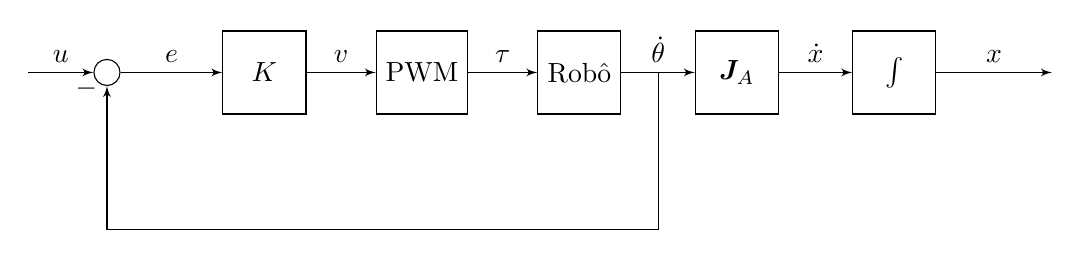
\begin{tikzpicture}[auto, node distance=2cm,>=latex']
    % We start by placing the blocks
    \node [input, name=input] {};
    \node [sum, right of=input] (sum) {};
    \node [block, right of=sum] (K) {$K$};
    \node [block, right of=K] (PWM) {PWM};
    \node [block, right of=PWM] (Robo) {Robô};
    \node [block, right of=Robo] (JA) {$\bm{J}_A$};
    \node [block, right of=JA] (Integral) {$\int$};
    \node [tmp, below of=K] (tmp1){};
    \node [output, right of=Integral] (output) {};

    % Once the nodes are placed, connecting them is easy. 
    \draw [draw,->] (input) -- node {$u$} (sum);
    \draw [->] (sum) -- node {$e$} (K);
    \draw [->] (K) -- node {$v$} (PWM);
    \draw [->] (PWM) -- node [name=tau] {$\tau$} (Robo);
    \draw [->] (Robo) -- node [name=dtheta] {$\dot{\theta}$} (JA);
    \draw [->] (JA) -- node {$\dot{x}$} (Integral);
    \draw [->] (Integral) -- node [name=x] {$x$}(output);
    \draw [->] (dtheta) |- (tmp1)-| node[pos=0.99] {$-$} (sum);
\end{tikzpicture}
\caption{Diagrama de Blocos: Malha de Controle de Velocidade a nível de juntas.}
\label{fig:controlejuntas}
\end{figure}


Portanto é possível implementar o controle cinemático segundo o diagrama \ref{fig:controlecinematico} 	

\begin{figure}[h!]
\centering
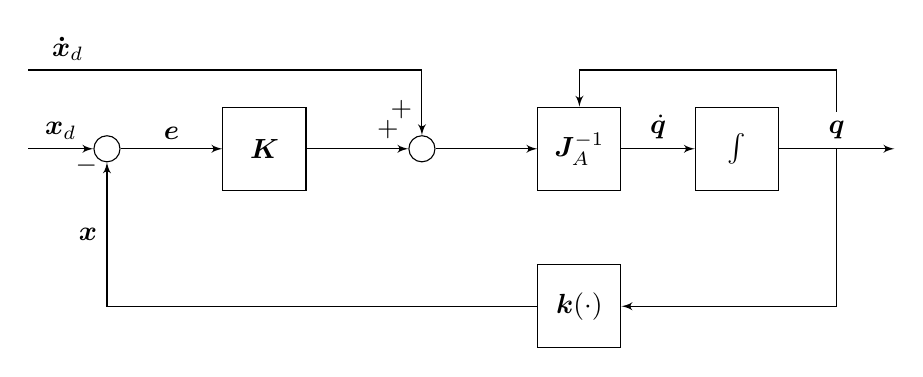
\begin{tikzpicture}[auto, node distance=2cm,>=latex']
    % We start by placing the blocks
    \node  [input, name=input2] {};
    \node at (0,-1) [input, name=input] {};
    \node [sum, right of=input] (sum) {};
    \node [block, right of=sum] (K) {$\bm{K}$};
    \node [sum, right of=K, node distance=2cm] (sum2) {};
    \node [tmp, above of =sum2, node distance=1cm] (tmp1){};
    \node [block, right of=sum2] (JA) {$\bm{J}_A^{-1}$};
    \node [block, below of=JA] (k) {$\bm{k}(\cdot)$};
    \node [block, right of=JA] (Integral) {$\int$};
    \node [tmp, above of=JA, node distance=1cm] (tmp2){};
    \node [output, right of=Integral] (output) {};

    % Once the nodes are placed, connecting them is easy. 
    \draw [draw,->] (input) -- node {$\bm{x}_d$} (sum);
    %\draw [draw,->] (input2) -- node {$u$} (sum2);
    \draw [draw,->] (input2) -- node [pos=0.1] {$\bm{\dot{x}}_d$} (tmp1)-| node [pos=0.8,anchor=left,left] {$+$} (sum2);
    \draw [->] (sum) -- node {$\bm{e}$} (K);
    \draw [->] (K) -- node {}  node[pos=0.8] {$+$} (sum2);
    \draw [->] (sum2) -- node [name=tau]  {} (JA);
    \draw [->] (JA) -- node [name=dtheta] {$\dot{\bm{q}}$} (Integral);
    \draw [->] (Integral) -- node [name=x] {$\bm{q}$}(output);
    \draw [->] (x) |- (k);
    \draw [->] (k) -| node[pos=0.99] {$-$} node [near end] {$\bm{x}$} (sum);
    \draw [->] (x) |- (tmp2) -| (JA);
    %\draw [->] (output) |- (tmp1)-| node[pos=0.99] {$-$} (sum);
\end{tikzpicture}
\caption{Diagrama de Blocos: Controle Cinemático Proporcional com FeedForward}
\label{fig:controlecinematico}
\end{figure}


Se $x$ é uma representação da posição e orientação e $x_d$ o valor desejado nessa representação, seja o erro no espaço operacional:
\begin{equation}
\bm{e} = \bm{x}_d - \bm{x}
\end{equation}

Derivando em relação ao tempo
\begin{equation}
\bm{\dot{e}} = \bm{\dot{x}}_d - \bm{\dot{x}}
\end{equation}
podemos escrever a partir da equação \ref{eq:jacoba}:
\begin{equation}
\bm{\dot{e}} = \bm{\dot{x}}_d - \bm{J}_a(\bm{q})\dot{\bm{q}}
\end{equation}
Sendo $\bm{x}_d(t)$ uma trajetória desejada, deseja-se que $\bm{x}$ atinja $\bm{x}_d(t)$ em $t \to \infty$ .
A entrada de controle para o sistema é um valor de $\bm{u} = \dot{\bm{q}}$, logo, assumindo que $\bm{J}_A(q)$ é quadrada e não singular, a escolha da lei de controle
\begin{equation}
\bm{u} = \bm{J}_A^{-1}(\bm{q})\bar{\bm{u}}
\end{equation}
leva ao sistema linear:
\begin{equation}
\dot{\bm{e}} = \dot{\bm{x}}_d - \bar{\bm{u}}
\end{equation}
Se for escolhido $\bar{\bm{u}}$:
\begin{equation}
\bar{\bm{u}} = \dot{\bm{x}}_d + \bm{K} (\bm{x}_d - \bm{x})
\end{equation}
obtem-se a seguinte dinâmica para o erro
\begin{equation}
\dot{\bm{e}} + \bm{K} \bm{e} = 0
\end{equation}

\section{Servo Visão}
A tarefa proposta na Servo Visão é controlar a posição e orientação do efetuador do manipulador, em relação a um alvo, usando características visuais extraidas de uma imagem. A câmera pode ser carregada pelo manipulador (montada no efetuador) ou colocada em um ponto fixo, observando tanto o efetuador como o alvo.

\subsection{Servo Visão Baseada em Posição}
Em um sistema de servo visão baseado em posição a posição e orientação do alvo com respeito a câmera $\bm{T}_{CT}$ é estimada. O problema de estimação da posição e orientação é discutido no apêndice ?.
Especifica-se uma posição desejada relativa ao sistema de coordenadas do alvo  $\bm{T}_{C^*T}$ e deseja-se determinar o movimento necessário para mover a câmera para a posição desejada, que chamamos de $\bm{T}_\delta$.

\begin{equation}
 \bm{T}_{CT} =  \bm{T}_\Delta \bm{T}_{C^*T}
\end{equation}

\begin{equation}
 \bm{T}_\Delta  =   \bm{T}_{CT} \bm{T}_{C^*T}^{-1}
\end{equation}
  \chapter{TETIS - Modelagem e Controle}


\section{Modelo}
O manipulador TETIS consiste basicamente de um braço planar de três elos com uma rotação adicional ao redor do eixo do plano. Também pode ser visto como um braço antropomórfico com uma junta de revolução adicional ao final da cadeia, com o eixo paralelo às duas anteriores. O projeto mecânico faz com que a extremidade do efetuador final não esteja exatamente alinhada com as juntas, o que é levado em conta no último elo. O esquema na figura \ref{fig:modelo_tetis} ilustra o modelo de elos e juntas. 
\begin{figure}[!ht]
\centering
  \includegraphics[width=0.9\linewidth]{./img/model2.png}
  \caption{Modelagem cinemática do manipulador TETIS e posicionamento dos sistemas de coordenadas}
  \label{fig:modelo_tetis}
\end{figure}%

\section{Cinemática Direta}
O primeiro passo ao modelar um manipulador robótico é encontrar a cinemática direta. Será utilizada a convenção de Denavit-Hartenberg para posicionar os sistemas de coordenadas e obter os parâmetros. Seguindo os passos descritos em \ref{sec:denavit} os sistemas de coordenadas foram posicionados da seguinte forma:

\begin{itemize}
\item Eixo $\vec{z}_0$ escolhido ao longo da Junta 1. Origem $O_0$ escolhida arbitrariamente de modo a coincidir com $O_1$ por simplicidade.  
\item Eixo $\vec{z}_1$ escolhido ao longo da Junta 2. Origem $O_1$ na intersecção entre $\vec{z}_0$ e $\vec{z}_1$. Eixo $\vec{x}_1$ na direção normal ao plano definido por $\vec{z}_0$ e $\vec{z}_1$ pois se interceptam. O sentido foi arbitrariamente escolhido na direção de avanço da cadeia por simplicidade.
\item Eixo $\vec{z}_2$ escolhido ao longo da Junta 3. Origem $O_2$ na junta 3 pois $\vec{z}_2$ e $\vec{z}_1$ são paralelas. Eixo $\vec{x}_2$ escolhido arbitrariamente ao longo de $\vec{x}_1$ pois a normal comum entre $\vec{z}_2$ e $\vec{z}_1$ não é unicamente definida.
\item Eixo $\vec{z}_3$ escolhido ao longo da Junta 4. Origem $O_3$ na junta 3 pois $\vec{z}_3$ e $\vec{z}_2$ são paralelas. Eixo $\vec{x}_3$ escolhido arbitrariamente ao longo de  $\vec{x}_2$ pois a normal comum entre $\vec{z}_3$ e $\vec{z}_2$ não é unicamente definida.
\item Como não existe junta 5, eixo $\vec{z}_4$ definido arbitrariamente. Origem $O_4$ na extremidade do efetuador final. Eixo $\vec{x}_4$ normal ao eixo $\vec{z}_3$.
\end{itemize}

A partir dos eixos posicionados conforme a figura \ref{fig:modelo_tetis} é possível obter os parâmetros na tabela \ref{tab:dh_tetis}. 


\begin{table}[h!]
\centering
\caption{Parâmetros Denavit–Hartenberg para manipulatodor Tetis}
\label{tab:dh_tetis}
\begin{tabular}{rrrrr} \hline
Elo & $a_i$ & $\alpha_i$ & $d_i$  & $\theta_i$ \\ \hline
1   & 0     & $\pi/2$    & 0      & $\theta_1$ \\
2   & $E_3$ & 0          & 0      & $\theta_2$ \\
3   & $E_4$ & 0          & 0      & $\theta_3$ \\
4   & $E_5$ & $-\pi/2$   & $-M_5$ & $\theta_4$ \\ \hline
\end{tabular}
\end{table}


\begin{itemize}
\item $a_1 = 0$  e $d_1 = 0$ pois $O_0$ e $O_1$ coincidem. $\alpha_1 = \pi/2$ ângulo entre $\vec{z}_0$ e $\vec{z}_1$ ao redor de $\vec{x}_1$.
\item $a_2 = E_3$ é a distância entre $\vec{z}_1$ e $\vec{z}_2$ ao longo de $\vec{x}_2$ que corresponde ao comprimento do elo 2. $\vec{z}_1$ e $\vec{z}_2$ são sempre paralelos logo $\alpha_2 = 0$. A distância $d_2$ entre $\vec{x}_1$ e $\vec{x}_2$ ao longo de $\vec{z}_1$ é zero. 

\item $a_3 = E_4$ é a distância entre $\vec{z}_2$ e $\vec{z}_3$ ao longo de $\vec{x}_3$ que corresponde ao comprimento do elo 3. $\vec{z}_2$ e $\vec{z}_3$ são sempre paralelos logo $\alpha_3 = 0$. A distância $d_3$ entre $\vec{x}_2$ e $\vec{x}_3$ ao longo de $z_2$ é zero. 

\item $a_4 = E_5$ é a distância entre $\vec{z}_3$ e $\vec{z}_4$ ao longo de $\vec{x}_4$. $\alpha_4 = -\pi/2$ é o ângulo entre $\vec{z}_3$ e $\vec{z}_4$ ao redor de $\vec{x}_4$, sendo portanto negativo. $d_4 = -M_5$ é a distância entre $\vec{x}_3$ e $\vec{x}_4$ ao longo de $\vec{z}_3$. 
\end{itemize}

Considerando a posição inicial da figura \ref{fig:modelo_tetis} todos os ângulos $\theta_i$ são dados diretamente pelas variáveis de junta, sem \textit{offsets}. 


Obtemos a partir da equação \eqref{eq:transform_dh} as transformações homogêneas entre sistemas de coordenadas consecutivos:
%\begin{align*}
%\bm{R}_{01} =
%\m{c_1 & 0 & s_1   \\
%   s_1 & 0 & -c_1  \\
%   0   & 1 &    0  \\} 
%& & \vec{\bm{p}}_{01} = 0
%\end{align*}
%\begin{align*}
%R_{12} = 
%\m{c_2 & -s_2 &  0  \\
%   s_2 &  c_2 &  0  \\
%   0   &    0 &  1  \\} 
%\end{align*}
%\begin{align*}
%R_{23} = 
%\m{c_3 & -s_3 &  0  \\
%   s_3 &  c_3 &  0  \\
%   0   &    0 &  1  \\} 
%\end{align*}
%\begin{align*}
%R_{34} = 
%\m{c_4 &  0 & -s_4  \\
%   s_4 &  0 &  c_4  \\
%   0   & -1 &    0  \\} 
%\end{align*}


%\begin{equation}
%\bm{R}_{04} = 
%\m{
%	c_1 c_{234} & -s_1 & -c_1 s_{234} \\
%	s_1 c_{234} & -c_1 & -s_1 s_{234} \\
%		s_{234} &    0 & 	  c_{234}
%}
%\end{equation}

\begin{align*}
{T}_{01} = 
\m{c_1 & 0 & s_1 &  0 \\
   s_1 & 0 & -c_1 & 0 \\
   0   & 1 &    0 & 0 \\
   0   & 0 &    0 & 1}
& &
{T}_{12} =  \m{c_2 & -s_2 &  0 & E_3 c_2 \\
   s_2 &  c_2 &  0 & E_3 s_2  \\
   0   &    0 &  1 & 	   0  \\
   0   &    0 &  0 &       1} 
\end{align*}

\begin{align*}
{T}_{23} = 
\m{c_3 & -s_3 &  0 & E_4 c_3 \\
   s_3 &  c_3 &  0 & E_4 s_3  \\
   0   &    0 &  1 & 	   0  \\
   0   &    0 &  0 &       1}
& &
{T}_{34} = 
\m{c_4 &    0 &  -s_4 & E_5 c_4 \\
   s_4 &    0 &   c_4 & E_5 s_4 \\
   0   &   -1 &     0 & 	-M_5 \\
   0   &    0 &     0 &       1}
\end{align*}


\begin{equation} \label{eq:cine_direta}
{T}_{04} = {T}_{01} {T}_{12}  {T}_{23} {T}_{34} = 
\m{
   c_1 c_{234} & -s_1 & -c_1 s_{234} & -M_5 s_1 + E_4 c_{23}c_1 + E_3 c_1 c_2 + E_5 c_{234} c_1 \\
   s_1 c_{234} & -c_1 & -s_1 s_{234} &   M_5 c_1+E_4 c_{23} s_1 + E_3 c_2 s_1 + E_5 c_{234} s_1 \\
   s_{234}     &    0 &      c_{234} &					     E_4 s_{23} + E_3 s_2 + E_5 s_{234} \\
   0   &    0 &     0 &      												   1
} 
\end{equation}

Definindo ${T}_{b0} = {I}$ e ${T}_{4e} = {I}$, pela equação \eqref{eq:base_efetuador} temos
\begin{equation}
{T}_{be} ({q}) = {T}_{04}({q})
\end{equation}


\section{Espaço das Juntas e Operacional}
Antes de tratar de estratégias de controle é necessário definir o espaço operacional e o espaço das juntas,  sob os quais serão aplicadas as leis de controle. 
Como trata-se de um manipulador 4-DOF de temos que o vetor do espaço operacional tem dimensão $(4 \times 1)$ dado por 
\begin{equation} \label{eq:operational_space}
{x_e} = \m{{p}_e \\ \phi_e}
\end{equation}
onde o vetor ${p}_e$ descreve a posição cartesiana representada no referencial da base:
\begin{equation}
{p}_e = \m{x \\ y \\ z}
\end{equation}
e $\phi_e$ é o grau de liberdade de orientação \textit{pitch}, dado por
\begin{equation} \label{eq:orientacao}
\phi_e = -(\theta_2 + \theta_3 + \theta_4)
\end{equation}

O espaço das juntas é definido por 
\begin{equation} \label{joint_space}
{q} = \m{q_1 \\ q_2 \\ q_3 \\ q_4} = \m{\theta_1 \\ \theta_2 \\ \theta_3 \\ \theta_4  }
\end{equation} 
pois todas as juntas são de revolução.

\section{Cinemática Diferencial}

\subsection{Jacobiano Analítico}
A partir da cinemática direta em \eqref{eq:cine_direta} e da equação \ref{eq:jacob_pos} podemos obter o Jacobiano de posição para o manipulador diferenciando a equação em relação as variáveis de junta. 
\begin{equation}
{p}_e = \m{x \\ y \\ z} =
\m{
   -M_5 s_1 + E_4 c_{23}c_1 + E_3 c_1 c_2 + E_5 c_{234} c_1 \\
     M_5 c_1+E_4 c_{23} s_1 + E_3 c_2 s_1 + E_5 c_{234} s_1 \\
   						 E_4 s_{23} + E_3 s_2 + E_5 s_{234} \\
}
\end{equation}

\begin{equation}
({J}_{ap})_b = 
\m{
	\ddfrac{\partial x}{\partial q_1} & \ddfrac{\partial x}{\partial q_2} & \ddfrac{\partial x}{\partial q_3} & \ddfrac{\partial x}{\partial q_4}  \\
	\ddfrac{\partial y}{\partial q_1} & \ddfrac{\partial y}{\partial q_2} & \ddfrac{\partial y}{\partial q_3} & \ddfrac{\partial x}{\partial q_4}  \\
	\ddfrac{\partial z}{\partial q_1} & \ddfrac{\partial z}{\partial q_2} & \ddfrac{\partial z}{\partial q_3} & \ddfrac{\partial z}{\partial q_4}  \\
}
\end{equation}
onde
\begin{align*}
&\frac{\partial x}{\partial q_1} =& - M_5c_1 - E_4c_{23}s_1 - E_3c_2s_1 - E_5c_{234}s_1  \\
&\frac{\partial x}{\partial q_2} =& -c_1(E_4s_{23}+E_3s_2+E_5s_{234}) \\
&\frac{\partial x}{\partial q_3} =& -c_1(E_4s_{23}+E_5s_{234}) \\
&\frac{\partial x}{\partial q_4} =& -E_5s_{234}c_1 \\
&\frac{\partial y}{\partial q_1} =& -M_5s_1+E_4c_{23}c_1+E_3c_1c_2+E_5c_{234}c_1 \\
&\frac{\partial y}{\partial q_2} =& -s_1(E_4s_{23}+E_3s_2+E_5s_{234}) \\
&\frac{\partial y}{\partial q_3} =& -s_1(E_4s_{23}+E_5s_{234}) \\
&\frac{\partial y}{\partial q_4} =& -E_5s_{234}s_1 \\ 
&\frac{\partial z}{\partial q_1} =& 0 \\ 
&\frac{\partial z}{\partial q_2} =& E_4c_{23}+E_3c_2+E_5c_{234} \\
&\frac{\partial z}{\partial q_3} =& E_4c_{23}+E_5c_{234}\\
&\frac{\partial z}{\partial q_4} =& E_{5}c_{234} 
\end{align*}

A partir de \ref{eq:jacob_or} e de \ref{eq:orientacao} podemos calcular o Jacobiano de orientação
\begin{equation}
{J}_{a\phi}({q}) = \frac{\partial \phi_e}{\partial {q}} = \m{0 & -1 & -1 & -1}
\end{equation}
 
Em alguns modos como controle por servo visão e no controle manual com joystick é interessante fazer o controle no referencial do efetuador, portanto precisamos representar o Jacobiano de posição no referencial do efetuador como $({J}_{ap})_e = {R}_{be}^T ({J}_{ap})_b$.  

\begin{equation}
({J}_{ap})_e =  
\m{
    -M_5c_{234} & E_3s_{34}+E_4s_4 & E_4s_4 & 0 \\
    E_4c_{23}+E_3c_2+E_5c_{234} & 0 & 0 & 0 \\
    M_5s_{23} &  E_5+E_3c_{34}+E_4c_4 & E_5+E_4c_4 & E_5 
}
\end{equation}


%A partir daqui, para simplificar a notação, sempre será referenciado o Jacobiano Analitico no referencial da base $(\bm{J}_A)_0$  como  $\bm{J}_0$ e o Jacobiano Analítico no referencial do efetuador $(\bm{J}_A)_N$ como $\bm{J}_N$.

%\section{Singularidades}

\section{Malha Aberta no Espaço Operacional} 
Este é um modo em malha aberta, onde o sinal de entrada no controlador é de velocidade no referencial da base ou do efetuador, ou seja a velocidade linear ${\dot{p}}_d$. Utiliza-se a equação \eqref{eq:jacob_pos} para calcular a velocidade de cada junta. 

\begin{figure}[h!]
\centering
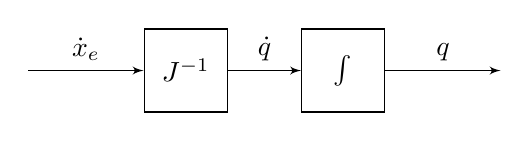
\begin{tikzpicture}[auto, node distance=2cm,>=latex']
    % We start by placing the blocks
    \node [input, name=input] {};
    \node [block, right of=input] (J) {$J^{-1}$};
    \node [block, right of=J] (Integral) {$\int$};
    \node [output, right of=Integral] (output) {};

    \draw [draw,->] (input) -- node {$\dot{{x}}_e$} (J);
    \draw [->] (J) -- node {${\dot{q}}$} (Integral);
    \draw [->] (Integral) -- node [name=x] {${q}$}(output);
\end{tikzpicture}
\caption{Diagrama de Blocos: Modo de velocidade do Espaço Operacional}
\label{fig:vel_op}
\end{figure}


\subsection{Sistema de coordenadas da Base} \label{sec:openloopbase}
Quando o controle é feito no referencial da base ${\dot{x}}_d$ é velocidade desejada expressa no referencial da base e utiliza-se $({J}_{a})_e$.
\begin{equation}
{u} = {\dot{q}}_d = ({J}_{a})_b^{-1} ({\dot{x}}_d)_e
\end{equation}
\subsection{Sistema de coordenadas do Efetuador} \label{sec:openloopefct}
Quando o controle é feito no referencial do efetuador ${\dot{x}}_d$ é velocidade desejada expressa no referencial do efetuador e utiliza-se $({J}_{a})_e$.
\begin{equation}
{u} = {\dot{q}}_d = ({J}_{a})_e^{-1} ({\dot{x}}_d)_e
\end{equation}
onde 
\begin{equation}
{\dot{x}}_d = \m{{\dot{p}}_d \\ 0}
\end{equation}

\section{Controle de Posição no Espaço das Juntas} \label{sec:position_joint}
O controle de posição no espaço das juntas consiste em uma realimentação com controle proporcional individual para cada junta. Considerando que as juntas sejam modeladas como integradores, o diagrama \ref{fig:pos_juntas} mostra a malha de controle.

\begin{figure}[h!]
\centering
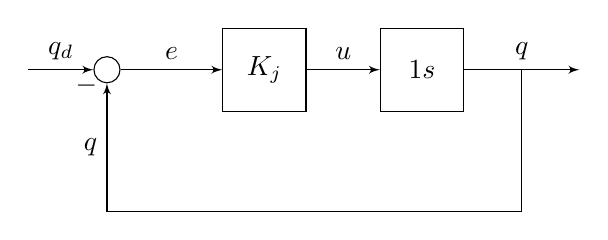
\begin{tikzpicture}[auto, node distance=2cm,>=latex']
    % We start by placing the blocks
    \node [input, name=input] {};
    \node [sum, right of=input] (sum) {};
    \node [block, right of=sum] (controller) {${K}_j$};
    \node [block, right of=controller] (system) {$\ddfrac{1}{s}$};
    % We draw an edge between the controller and system block to 
    % calculate the coordinate u. We need it to place the measurement block. 
    \draw [->] (controller) -- node[name=u] {${u}$} (system);
    \node [output, right of=system] (output) {};
    \node [tmp, below of=u] (tmp1) {};

    % Once the nodes are placed, connecting them is easy. 
    \draw [->] (system) -- node [name=s] {${q}$}(output);
    \draw [draw,->] (input) -- node {${q_d}$} (sum);
    \draw [->] (sum) -- node {${e}$} (controller);
    \draw [->] (s) |- (tmp1)-| node[pos=0.99] {$-$} node [near end] {${q}$} (sum);
       %\draw [->] (measurements) -| node[pos=0.99] {$-$} 
       % node [near end] {$\bm{q}_m$} (sum);
\end{tikzpicture}
\caption{Diagrama de Blocos: Modo de Posição no Espaço das Juntas}
\label{fig:pos_juntas}
\end{figure}

A lei de controle é dada por 
\begin{equation}
{u} = {K}_j ({q}_d - {q})
\end{equation}
onde ${K_j} = k_j {I}$.

\section{Controle de Posição no Espaço Operacional} \label{sec:pos_operacional}
Para este modo considera-se o problema de \textit{set-point} para o controle de posição no espaço operacional conforme definido em \ref{eq:op_space}. Para referências constantes, ou seja, quando $\dot{{x}}_d = 0$ a lei de controle dada por
\begin{equation} \label{eq:lei_posicao}
{u} = ({J}_{a})_b^{-1} {K}_p ( ({x_d})_b - ({x_e})_b)
\end{equation}
é capaz de levar o ${e} \rightarrow 0$ quando $t \rightarrow \infty$.

\section{Controle Proporcional com Feedforward} \label{sec:pplusf}
Para o rastreamento de trajetória considera-se o problema de seguir um referência no referencial da base ${x}_d(t)$ que é função do tempo, conhecidos ${x}_d(t)$ e ${\dot{x}}_d(t)$. Para levar o erro assintoticamente a zero, utiliza-se uma lei de controle proporcional com \textit{feedforward} utilizando a inversa do Jacobiano Analítico. Conforme mostrado na Seção \ref{sec:controle_cinematico}, a lei de controle dada por 
\begin{equation}
{u} = ({J}_{a})_b^{-1} (\dot{{x}}_d + {K}_t ({x_d} - {x_e}))
\end{equation} 
é capaz de levar o erro assintoticamente a zero pois a dinâmica fica 
\begin{equation}
\dot{{e}} + {K} {e} = 0
\end{equation}
O algoritmo de controle pode ser resumido por:
\begin{align}
{e} &= ({x}_d)_b- ({x_e})_b  \label{eq:error_pf}\\
{\bar{u}} &= {K}_t {e} + ({\dot{x}}_d)_b \\
{u} &= ({J}_a)_b^{-1} {\bar{u}}
\end{align}

%\begin{algorithm}
%\caption{<your caption for this algorithm>}
%\begin{algorithmic}
%\State $t = getTime()$
%\State $t = getTime()$
%\If {$i\geq maxval$}
%%    \State $i\gets 0$
%\Else
%    \If {$i+k\leq maxval$}
%        \State $i\gets i+k$
%    \EndIf
%\EndIf
%\end{algorithmic}
%\end{algorithm}

\section{Controle por Servo Visão} \label{sec:servo_vision}
O controle por servo visão no manipulador TETIS é feito através de uma configuração \textit{eye-in-hand}, onde a câmera é montada no efetuador final do manipulador, utilizando a abordagem de Servo Visão Baseada em Posição (PBVS). Na seção \ref{sec:minoru} é descrita a câmera utilizada. Trata-se de uma câmera estereoscópica, no entanto será utilizada apenas um dos sensores.

%\begin{figure}[H]
%\centering
%\begin{subfigure}{.5\textwidth}
%  \centering
%  \includegraphics[width=\linewidth]{./img/manip_zoom.png}
%  \caption{Efetuador com câmera}
%  \label{fig:efetuador}
%\end{subfigure}%
%\begin{subfigure}{.5\textwidth}
%  \centering
%  \includegraphics[width=0.8\linewidth]{./img/minoru.jpg}
%  \caption{Minoru Camera}
%  \label{fig:minoru}
%\end{subfigure}
%\label{fig:efet_minoru}
%\caption{Efetuador e câmera Minoru}
%\end{figure}


O objetivo é deste modo de controle é rastrear um alvo, que é representado por um QR code como o da figura \ref{fig:camera_target}. Deseja-se que o efetuador rastreie sempre a orientação normal ao plano do alvo.

A matriz de calibração ${K}$ da equação \eqref{eq:camera_projection} obtida através do processo descrito em \citep{visp_camera_calibration} é:

\begin{equation}
{K} = \m {
	f/\rho_w & 0 & u_0 \\
	0        & f/\rho_h &v_0 \\
	0 & 0 & 1 \\
}
=
\m{
	877.62 	& 0 		& 306.53 \\
	0  		& 880.32 	& 210.12 \\
	0   	& 0 		& 1 \\	
}	
\end{equation}

Observando que o referencial da câmera e do efetuador são dados pela figura \ref{fig:camera_ref}, podemos chegar a seguinte transformação homogênea

\begin{equation} \label{eq:tec}
{T}_{ec} = \m{
	0 & 0 & 1 & -30 \\
	0 & -1 & 0 & 101 \\
	1 &  0 & 0 & -43 \\
	0 &  0 & 0 &  1
}
\end{equation}

\begin{figure}[!h]
  \centering
  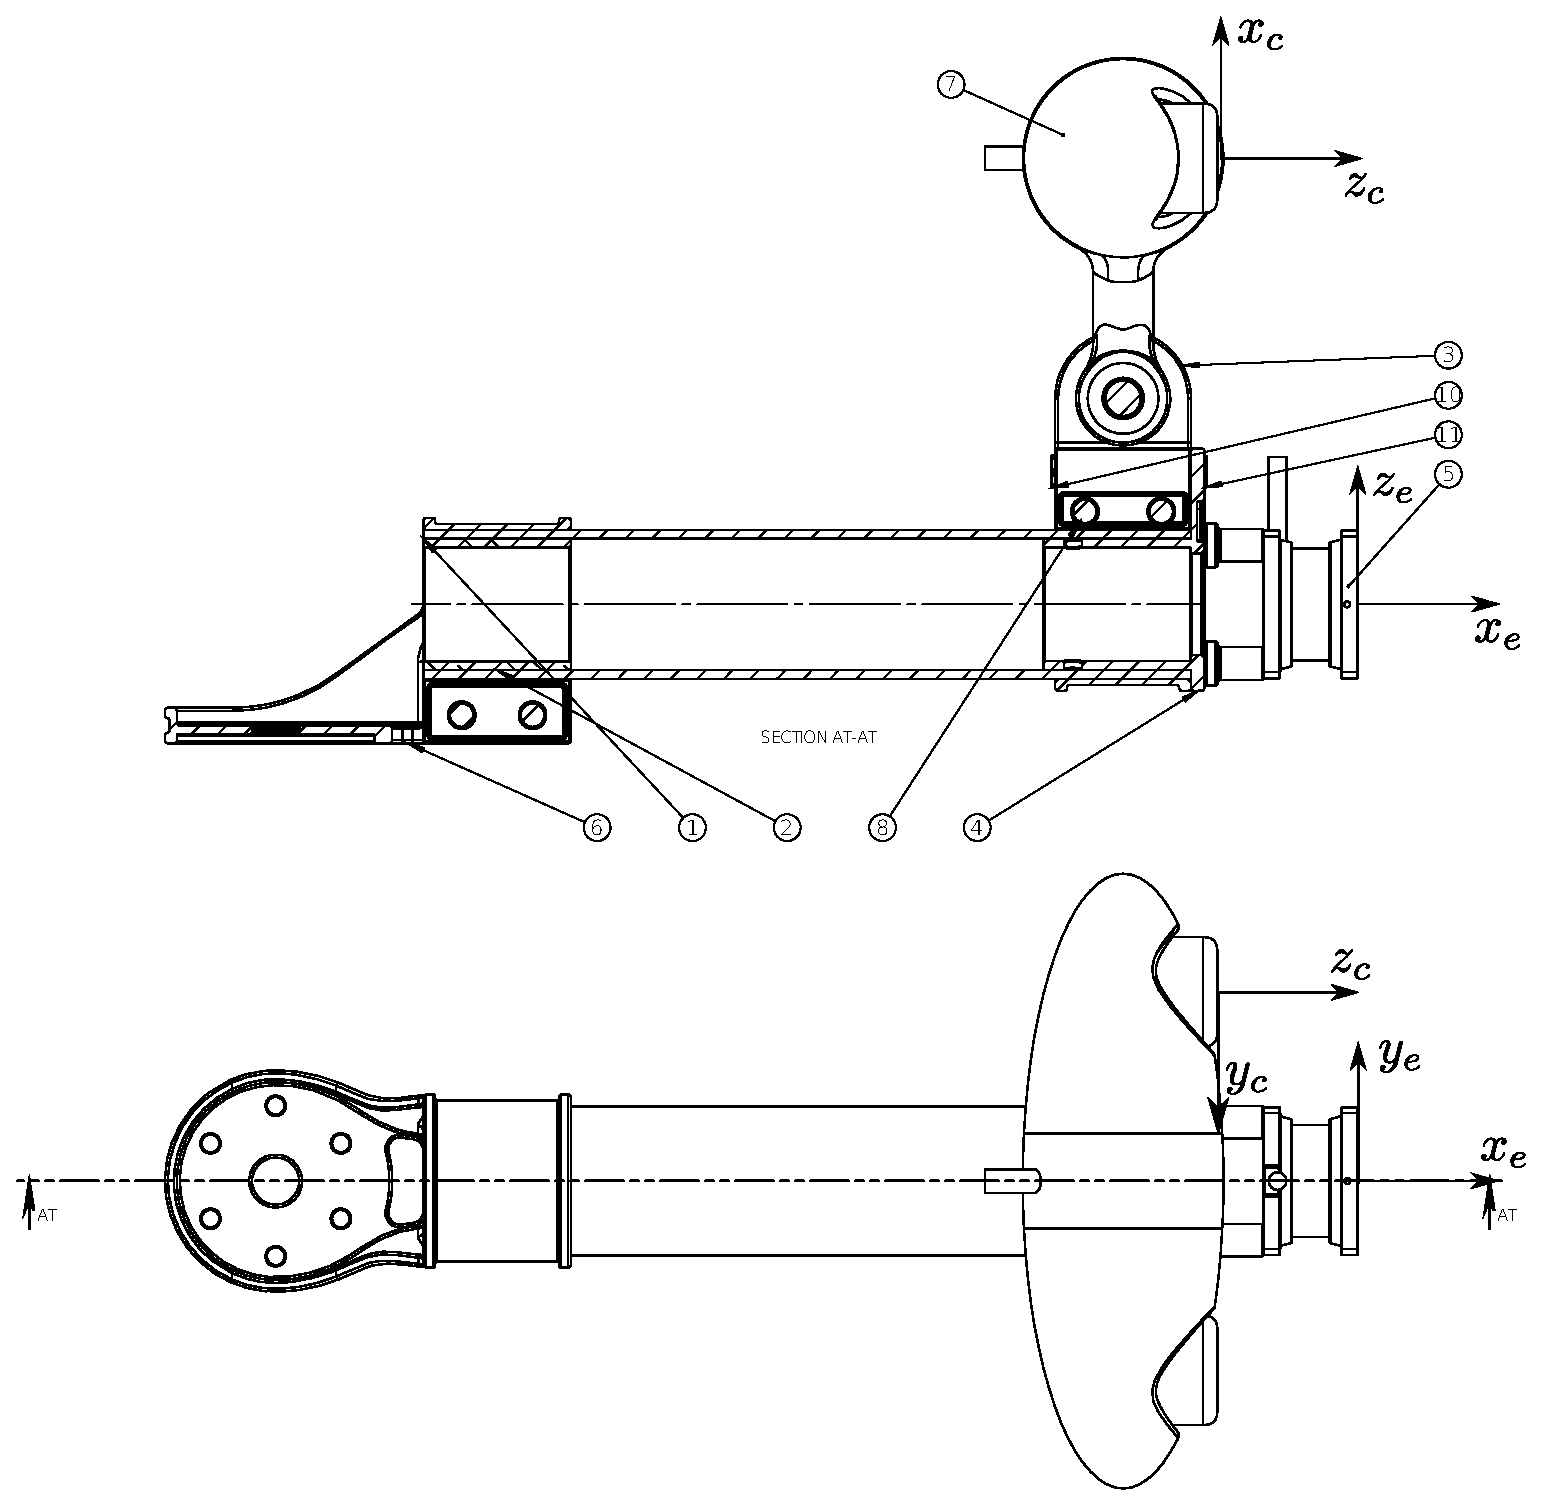
\includegraphics[width=0.8\linewidth]{./img/effector2}
  \caption{Sistemas de coordenadas da câmera e do efetuador}
  \label{fig:camera_ref}
\end{figure}

\begin{figure}[!h]
  \centering
  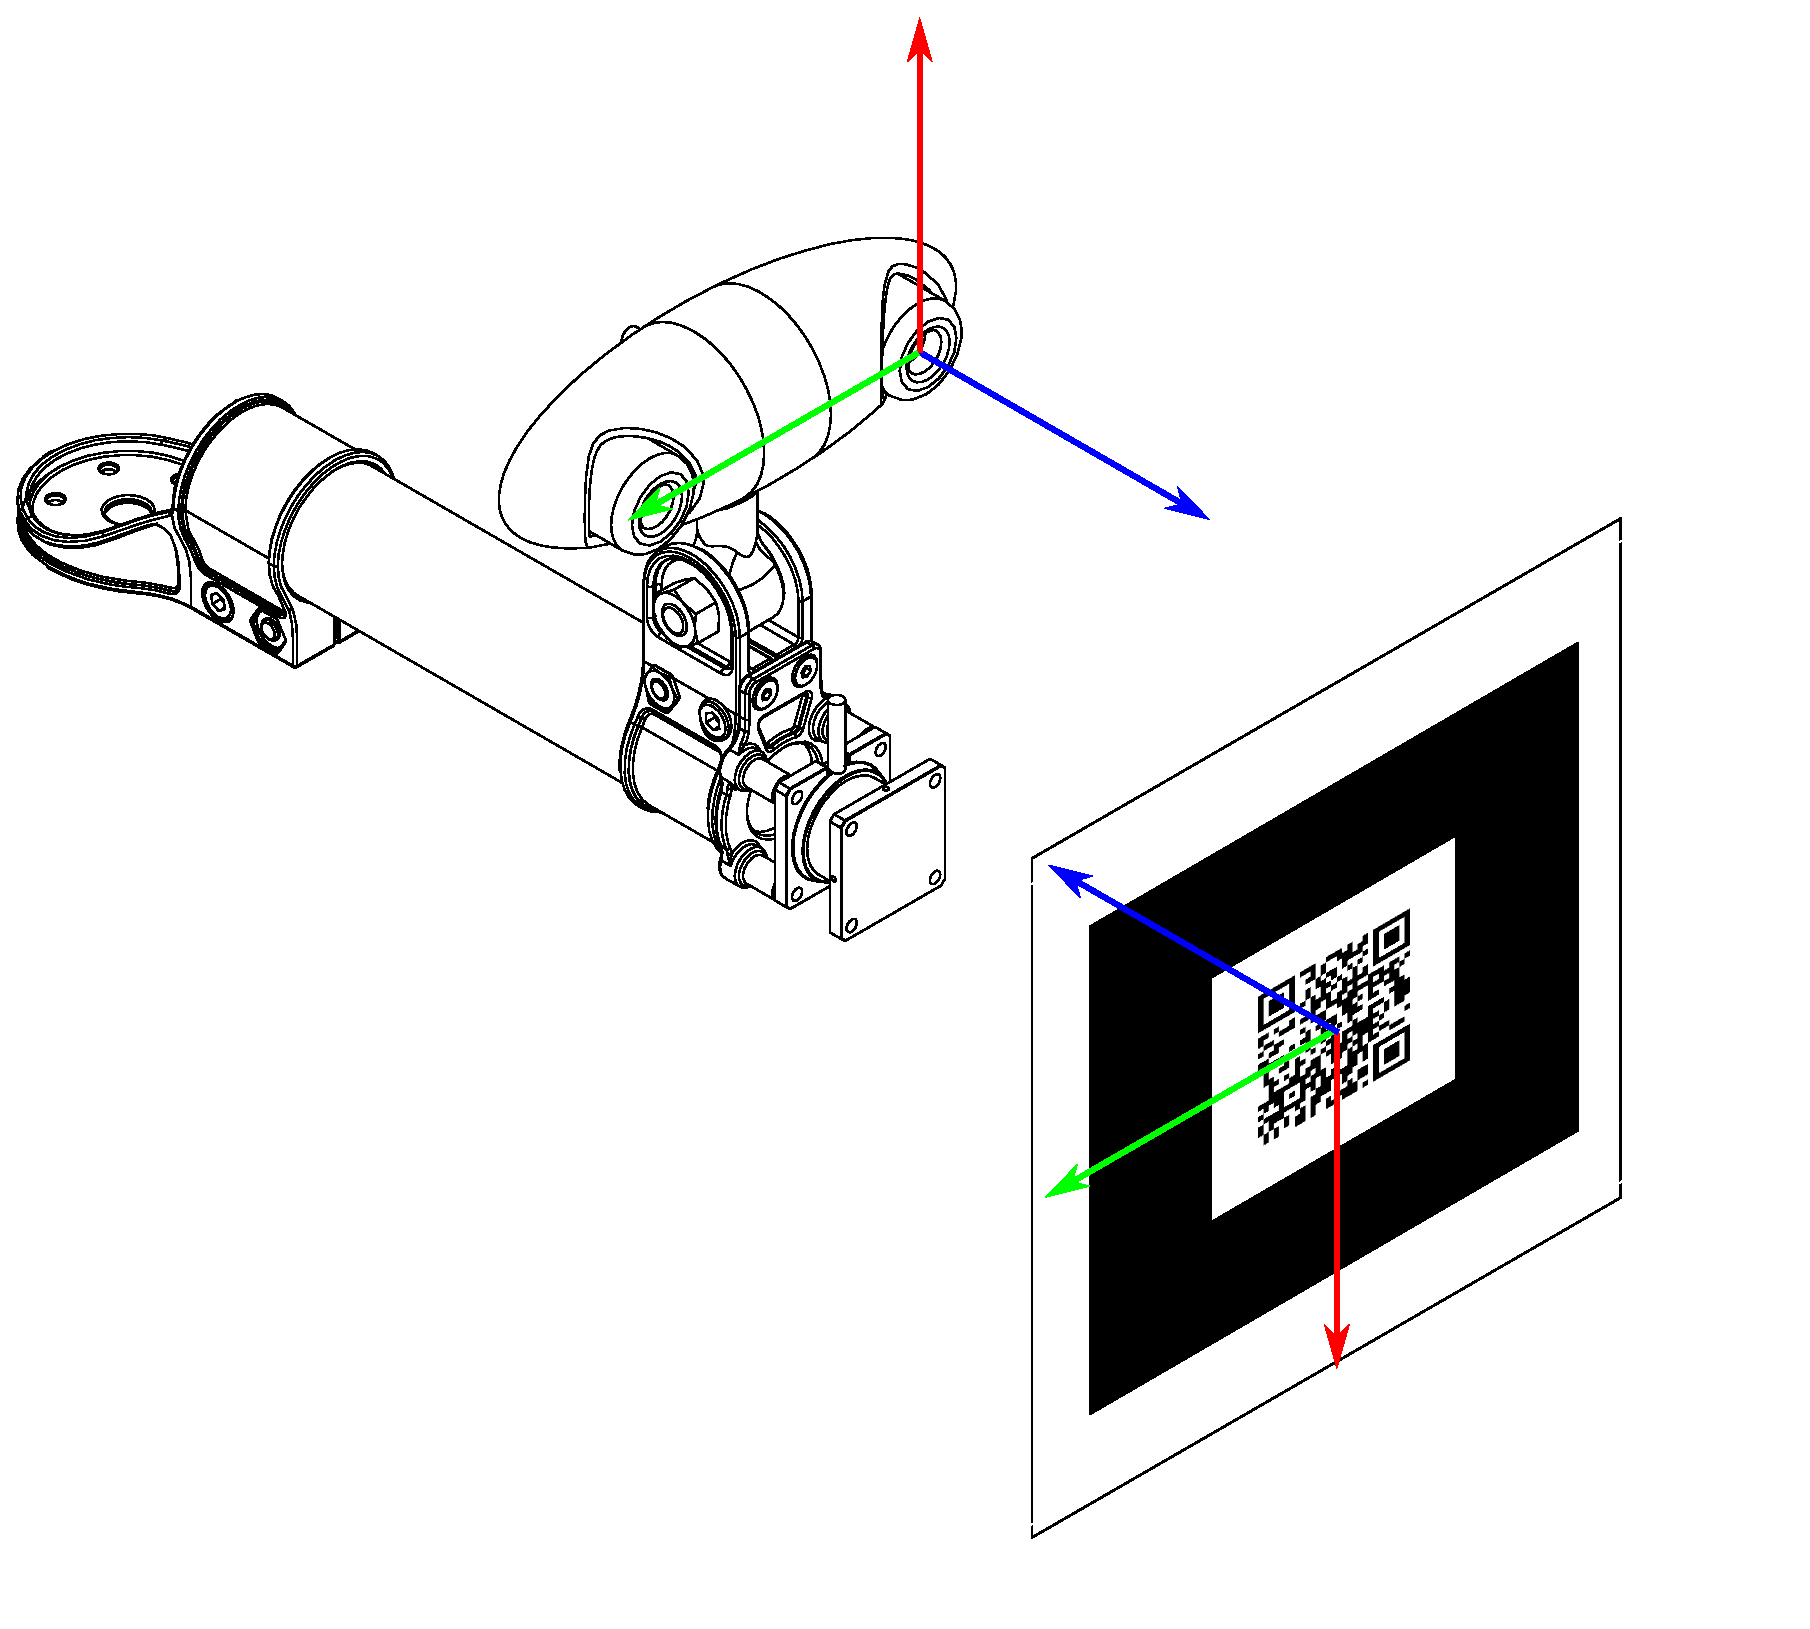
\includegraphics[width=0.8\linewidth]{./img/camera_target}
  \caption{Sistemas de coordenadas da câmera e do alvo}
  \label{fig:camera_target}
\end{figure}


Para a servo visão baseada em posição, foi utilizada uma lei de controle proporcional
\begin{equation} \label{eq:lei_posicao}
{u} = ({J}_{a})_e^{-1} {K}_t [({x}_t)_e - ({x_e})_e]
\end{equation}
onde ${x}_t$ e ${x_e}$ estão representados no referencial do efetuador. Portanto precisamos saber a posição e orientação ${x}_t$ do alvo em relação ao efetuador
\begin{equation}
{T}_{et} = {T}_{ec} {T}_{ct}
\end{equation}
onde ${T}_{ec}$ é dado por \eqref{eq:tec} e ${T}_{ct}$ obtemos através de algoritmos de estimação de posição e orientação a partir de visão computacional. 

\begin{equation}
({x}_t)_e = \m{ ({p}_t)_e \\ \phi_t }
\end{equation}
onde $({p}_t)_e$ é o vetor de translação que pode ser obtido diretamente de ${T}_{ec}$ e  $\phi_t$ é a orientação, que pode ser obtido de duas formas.


%TODO
A primeira alternativa é obter a rotação em torno do eixo $x$ (\textit{pitch}) em relação ao referencial do efetuador, extraído de ${T}_{et}$. No entanto essa opção não permite que o alvo seja rotacionado em torno de ${z}_c$, pois a rotação em torno de ${x}_c$ não mais representará a inclinação do plano do alvo em relação a posição inicial, que faz o efetuador rastrear a direção normal ao alvo. A figura \ref{fig:projection} ilustra isso. 

Portanto, optou-se pela segunda alternativa. Projeta-se o eixo do alvo $({z}_t)_c$, representado do referencial da câmera, no plano $({z}_{t_0})_c \times ({x}_{t_0})_c$, onde $({z}_{t0})_c$ indica o eixo de coordenadas do alvo $z_t$ em sua posição inicial conforme a figura \ref{fig:camera_target}. Em seguida encontra-se o ângulo entre os vetores $({z}_{t_0})_c$ e $({z}_{t_0})_c$. 

\begin{figure}[!ht]
\centering
  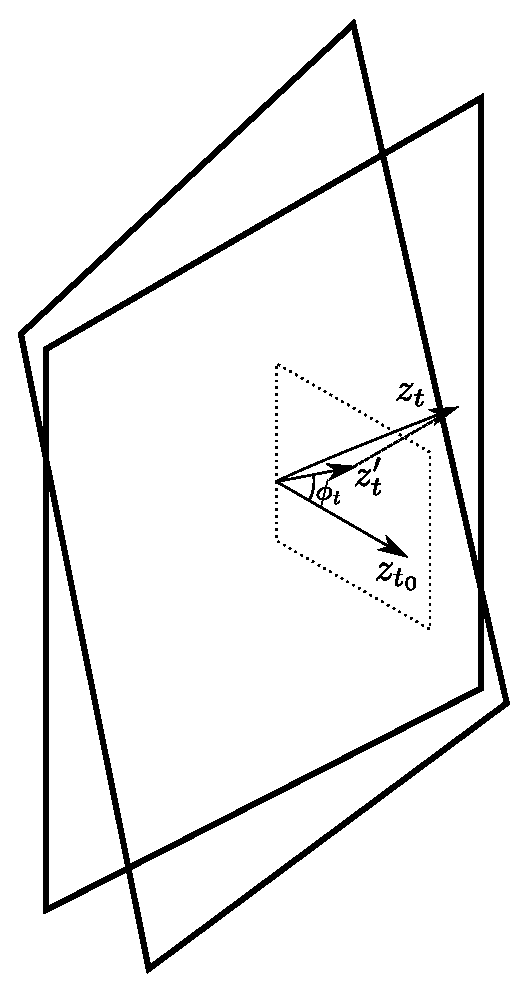
\includegraphics[width=0.3\linewidth]{./img/projection.eps}
  \caption{Caso em que a rotação em torno de ${x}_c$ não representa a inclinação do plano do alvo.}
  \label{fig:projection}
\end{figure}%


Dada a matriz de rotação ${R}_{ct_0}$, da câmera à posição inicial
\begin{equation}
{R}_{ct_0} = \m{ ({x}_{t_0})_c & ({y}_{t_0})_c  & ({z}_{t_0})_c} = 
\m{
	0 & 1 & 0 \\
	1 & 0 & 0 \\
	0 & 0 & -1
}
\end{equation}
é conhecida a normal ao plano do alvo é ${n} = {x}_{t_0} \times {z}_{t_0} =  {y}_{t_0} $. A matriz de projeção linear \citep{strang} de um vetor em um plano é dada por
\begin{equation}
{P} = {I} - {n} {n}^T,
\end{equation}
logo para ${n} = {y}_{t_0}$ temos 
\begin{equation}
{P} =  \m{
	 0  &   0  &   0 \\
     0  &   1  &   0 \\
     0  &   0  &   1
}.
\end{equation}

O vetor projetado no plano é dado por
\begin{equation}
{z'}_{t} = {P} {z}_{t},
\end{equation}
assim basta apenas encontrar o ângulo entre os vetores ${z'}_{t}$ e ${z}_{t_0}$, que pode ser calculado pela fórmula do Cosseno \citep{strang} 
\begin{equation}
\phi_t = \cos^{-1} \left( \frac{{z'}^T_{t} {z}_{t_0} } {||{z'}_{t}|| \; ||{z}_{t_0}||} \right)
\end{equation}
%\begin{align}
%(\bm{p}_t)_e &= (\bm{p}_c)_e + (\bm{p}_t)_e \\
%(\bm{p}_t)_e &= (\bm{p}_c)_e + \bm{R}_{ec} (\bm{p}_t)_c 
%\end{align}
Após obter os valores de $(p_t)_e$ e $\phi_t$, sabemos $(x_t)_e$ e controle se resume a:
\begin{align}
{e} &= ({x}_t)_e - ({x})_e \\
{\bar{u}} &= {K}_v {e}  \\
{u} &= ({J}_{a})_e^{-1} {e}
\end{align}

\section{Controle de Força} \label{sec:force}

Utilizando o sensor de força descrito em \ref{sec:optoforce}, montado no efetuador final do manipulador, deseja-se fazer o controle da força aplicada sobre uma superfície. 

A matriz de rotação do referencial do sensor para o referencial do efetuador, como definido em \ref{fig:modelo_tetis} é dada por

\begin{equation}
R_{es} = \m{
  0 & 0 & 1 \\
  0 & -1 & 0 \\
  1 & 0 & 0
}
\end{equation}

\subsection{Float}  \label{sec:forca_float}
Esse mode de controle de força consiste em configurar uma referência de controle de força ${f}_d = 0$, de modo que o efetuador do manipulador fique "flutuando", se movendo de forma sensível ao toque.

Primeiramente a força representada no referencial do sensor $({f})_s \in \mathbb{R}^3 $ é representada na base por $({f})_e = R_{es} ({f})_s$. Com ${f}_d = 0$, o erro fica
\begin{equation}
({e}_f)_e = - ({f})_e 
\end{equation}
Utilizando um controle proporcional:
\begin{align}
\bar{{u}}_f &= {K}_f ({e}_f)_e \\
\bar{{u}} &= \m{ \bar{{u}}_f & 0}^T\\
{u} &= ({J_a})_b^{-1} \bar{{u}}
\end{align}

\subsection{Approach} \label{sec:forca_approach}
Considera-se o problema de controle de força na direção de \textit{approach} para o manipulador robótico 4-DOF em questão. O objetivo de controle é resolver o problema de \textit{set-point}, ou seja, rastrear uma referência de força constante.

É possível modelar o ambiente (força de contato), ou seja, a placa de poliestireno, como uma mola linear, através da \textit{Lei de Hooke}: 
\begin{equation}
f = -k_s (x - x_s)
\end{equation}
onde $x$ é a posição do ponto de contato com a superfície e $x_s$ um ponto na superfície.

Considerando que o controle de força seja ativado somente após a etapa de contato com o ambiente onde será aplicada a força e que o controle de força é feito apenas na direção de approach (segundo o sistema de coordenadas $\bar{E}_e$, na direção $x$), pode-se utilizar a malha de controle mostrada na figura \ref{fig:controle_forca}.

É utilizada uma lei de controle com ação proporcional e integral:
\begin{equation}
\bar{u} = -K_s^{-1} (K_fe_f + K_i \int_0^t e_f(\tau)d\tau)
\end{equation}


\begin{figure}[h!]
\centering
\begin{tikzpicture}[auto, node distance=2cm,>=latex']
    % We start by placing the blocks
    \node [input, name=input] {};
    \node [sum, right of=input] (sum) {};
    \node [block, right of=sum] (Ks1) {$k_s^{-1}$};
    \node [block, right of=Ks1] (C) {$C(s)$};
    \node [blockbig=right:C] (J) [right=1cm of C] {$(J_a)_e^{-1}$};
    \node [block=right:J] (Integral) [right=1cm of J] {$\int$};
    \node [blockbig, right of=Integral] (DirKine) {${k}(\cdot)$};

	\node [tmp=below:J] (tmp0) [below left=-1.25cm and .7cm of J] {};
	\node [tmp=below:J] (tmp00) [below left=-2cm and 0.7cm of J] {};
	\node [tmp=below:J] (tmp000) [below left=-2cm and 0cm of J] {};

    \node [tmp=below:J] (tmp1) [below left=-1.5cm and 0.5cm of J] {};
    \node [tmp=below:J] (tmp2) [below left=-1.5cm and 0cm of J] {};

    \node [tmp=below:J] (tmp3) [below left=-1cm and 0.5cm of J] {};
    \node [tmp=below:J] (tmp4) [below left=-1cm and 0cm of J] {};

    \node [tmp=below:J] (tmp5) [below left=-0.5cm and 0.5cm of J] {};
    \node [tmp=below:J] (tmp6) [below left=-0.5cm and 0cm of J] {};

    \node [tmp=below:J] (tmpk0) [below right=-2cm and 0cm of DirKine] {};
	\node [tmp=below:J] (tmpk00) [below right=-2cm and 0.7cm of DirKine] {};
	\node [tmp=below:J] (tmpk000) [below right=-1.25cm and 0.7cm of DirKine] {};

    \node [tmp=below:J] (tmpk1) [below right=-1.5cm and 0.5cm of DirKine] {};
    \node [tmp=below:J] (tmpk2) [below right=-1.5cm and 0cm of DirKine] {};

    \node [tmp=below:J] (tmpk3) [below right=-1cm and 0.5cm of DirKine] {};
    \node [tmp=below:J] (tmpk4) [below right=-1cm and 0cm of DirKine] {};

    \node [tmp=below:J] (tmpk5) [below right=-0.5cm and 0.5cm of DirKine] {};
    \node [tmp=below:J] (tmpk6) [below right=-0.5cm and 0cm of DirKine] {};


    \node [block=right:DirKine] (ks) [right=1cm of DirKine] {$k_s$};
    \node [output, right of=ks] (output) {};

    % Once the nodes are placed, connecting them is easy. 
    \draw [draw,->] (input) -- node {$f_d$} (sum);
    \draw [->] (sum) -- node {$e_f$} (Ks1);
    \draw [->] (Ks1) -- node {} (C);
    %\draw [->] (C) -- node[name=u] {$u$} (tmp0);
    \draw [->] (J) -- node {${\dot{q}}$} (Integral);
    \draw [->] (Integral) -- node {${q}$} (DirKine);
    \node [block, below of=J] (measurements) {$H(s)$};
    %draw [->] (DirKine) -- node {} (ks);
    \draw [->] (ks) -- node [name=x] {$f$}(output);
    \draw [->] (x) |- (measurements);
    \draw [->] (measurements) -| node[pos=0.99] {$-$} 
        node[near end] {$f_m$} (sum);

    \draw [->] (C) -- (tmp0) -|  (tmp00) |- node[pos=0.65] {$x$} (tmp000);

    \draw [->] (tmpk0) -- node[pos=0.2] {$x$} (tmpk00) -|  (tmpk000) |-  (ks);
    \draw [->] (tmp1) -- node[pos=0] {$y$} (tmp2);
    \draw [->] (tmp3) -- node[pos=0] {$z$} (tmp4);
    \draw [->] (tmp5) -- node[pos=0] {$\phi$} (tmp6);

    \draw [->] (tmpk2) -- node[pos=0.3] {$y$} (tmpk1);
    \draw [->] (tmpk4) -- node[pos=0.3] {$z$} (tmpk3);
    \draw [->] (tmpk6) -- node[pos=0.3] {$\phi$} (tmpk5);
    %\draw [->] (x) |- (tmp1) -| node[pos=0.9] {$-$} (sum);
\end{tikzpicture}
\caption{Diagrama de Blocos: Malha de Controle de Força.}
\label{fig:controle_forca}
\end{figure}

O diagrama \ref{fig:controle_forca} pode ser simplificado se abstrairmos as outras dimensões que não a de approach, resultando em \ref{fig:controle_forca_simples}.

\begin{figure}[h!]
\centering
\begin{tikzpicture}[auto, node distance=2cm,>=latex']
    % We start by placing the blocks
    \node [input, name=input] {};
    \node [sum, right of=input] (sum) {};
    \node [block, right of=sum] (Ks1) {$k_s^{-1}$};
    \node [block, right of=Ks1] (C) {$C(s)$};
    \node [block, right of=C] (PWM) {$k_s$};
    \node [block, right of=PWM] (Robo) {$\ddfrac{1}{s}$};
    \node [tmp, below of=K] (tmp1){};
    \node [output, right of=Robo] (output) {};

    % Once the nodes are placed, connecting them is easy. 
    \draw [draw,->] (input) -- node {$f_d$} (sum);
    \draw [->] (sum) -- node {$e_f$} (Ks1);
    \draw [->] (Ks1) -- node {} (C);
    \draw [->] (C) -- node[name=u] {$u$} (PWM);
    \node [block, below of=u] (measurements) {$H(s)$};
    \draw [->] (PWM) -- node [name=tau] {} (Robo);
    \draw [->] (Robo) -- node [name=x] {$f$}(output);
    \draw [->] (x) |- (measurements);
    \draw [->] (measurements) -| node[pos=0.99] {$-$} 
        node[near end] {$f_m$} (sum);
    %\draw [->] (x) |- (tmp1) -| node[pos=0.9] {$-$} (sum);
\end{tikzpicture}
\caption{Diagrama de Blocos: Malha de Controle de Força Simplificada.}
\label{fig:controle_forca_simples}
\end{figure}

Considerando $H(s) = 1$
\begin{equation}
G(s) = \frac{k_p s + k_i}{s^2 + k_p s + k_i}
\end{equation}

Como o sinal vindo do sensor é bastante ruidoso, utiliza-se um filtro de primeira ordem com $f_c = 1$.
\begin{equation}
H(s) = \frac{1}{\tau s + 1}
\end{equation}
onde $\tau = 1/(2 \pi f_c) \approx 0.16$.

Ficamos com a função de transferência a seguir a partir da qual é possível sintonizar os parâmetros do controlador.
\begin{equation}
G(s) = \frac{k_p \tau s^2 + (k_p + \tau k_i)s + k_i}{\tau s^3 + s^2 + k_p s + k_i}
\end{equation}

Considerando que obtemos do sensor de força um vetor $({f})_s \in \mathcal{R}^3$, representado no referencial do sensor. O controle de força pode ser implementado a partir das seguintes equações:
\begin{align}
({f})_e &= {R}_{es} ({f})_s \\
({e}_f)_e &= {f}_d - ({f})_e \\
\end{align}
A estratégia de controle PI é dada por
\begin{equation}
\bar{{u}}_f = -{K}_s^{-1} ({K}_f ({e}_f)_e + {K}_i \int_0^t ({e}_f)_e (\tau)d\tau)\\
\end{equation}
Como ${u} \in \mathcal{R}^4$  e desejamos controlar somente a direção de \textit{approach}:
\begin{equation}
\bar{{u}} = \m{ {S}_f \bar{{u}}_f \\ 0} 
\end{equation}
onde 
\begin{equation}
{S}_f = \m{
  1 & 0 & 0 \\
  0 & 0 & 0 \\
  0 & 0 & 0
},
\end{equation}
portanto:
\begin{equation}
{u} = ({J_a})_e^{-1} \bar{{u}}
\end{equation}

%Especificações:
%\section{Controle Híbrido}
%Considerando o diagrama \ref{fig:controle_forca}, é possível suprir os graus de liberdade não controlados $y$, $z$ e $\phi$ %com outra lei de controle, como por exemplo o um Proporcional com Feedforward de modo a aplicar uma força na direção de %approach e traçar uma trajetória de na superfície em que a força está sendo aplicada. 

%\section{Master-Slave (Omni)}
%TODO

% TODO: TABELA COM LEIS DE CONTROLE E FONTE DOS DADOS 
  \chapter{Implementação}
A implementação dos algoritmos de controle detalhados nos capítulos anteriores for feita como extensão ao software RobotGUI desenvolvido pela equipe do LEAD-GSCAR, idealizado por Alex F. Neves Msc. 

\section{Motivação} 
Modular, genérico, ...

\section{Ferramentas}
Os seguintes softwares e \textit{frameworks} foram utilizados:

\begin{itemize}
\item Linux (Ubuntu) como Sistema Operacional
\item C++ como linguagem de programação
\item ROS como \textit{framework} principal utilizado o RobotGUI, fornecendo comunicação entre nós através de mensagens e serviços. Será descrito mais detalhadamente na próxima seção.
\item Qt como \textit{framework} para elaboração da interface gráfica. 
\end{itemize}

\section{ROS}

\section{Conceitos}

Primeiramente define-se como Computador Base aquele que será utilizado pelo operador para controlar e visualizar dados do robô. Define-se Computador Embarcado, ou do Robô aquele que está no robô conectado a todos os equipamentos, sensores e atuadores. O software executa módulos diferentes no robô e na base.

A arquitetura do RobotGUI baseia-se nos seguintes conceitos principais:

\begin{itemize}
\item \textbf{Components}: Lidam com a comunicação e processam dados no Computador Base. São essencialmente \textit{Nodelets} de ROS, podendo utilizar funcionalidades como comunicação através de mensagens e serviços, utilizar parametros e bibliotecas de ROS. Permitem maior modularidade pois comonentes podem ser inicializados independentemente do \textit{RobotGUI}.

\item \textbf{Tools:} São elementos gráficos da interface para o usuário. São utilizadas para interagir com o robô e visualizar informação. São criadas como \textit{plugins} para o ROS \textit{pluginlib} e independetes de qualquer biblioteca do ROS.

\item \textbf{Interação entre Compontents e Tools:} Tools e Components podem se conectar, quando isso ocorre eles interagem entre si a nível de "ponteiro para objeto". Essa conecção permite que o desenvolvimento da interface através do \textit{Qt} seja quase que independente do desenvolvimento do código que lida com hardware, lógica e comunicação.

\item \textbf{RobotGUI}
\end{itemize}


\section{Modos de Controle}

\subsection{Velocidade no Espaço Operacional}
\subsubsection{Base}
\subsubsection{Efetuador}
\subsection{Posição no Espaço das Juntas}
\subsection{Posição no Espaço Operacional}
\subsection{Rastreamento de Trajetória}
\subsection{Servo Visão}
\subsection{Força}
\subsubsection{Float}
\subsubsection{Approach}
\subsubsection{Híbrido}

  \chapter{Resultados e Discussões}

\section{Respostas das Juntas}
Para verificar se de fato são válidas as premissas assumidas na seção \ref{sec:controle_cinematico} para aplicação de uma estratégia de controle cinemático foi levantada para cada uma das juntas a resposta a uma onda quadrada tal que:
\[ u = A \sgn(\sin( 2\pi t/f)) \]
onde o período $T = 1/f = 1s$ e a amplitude $A = 0.5 rad/s$

\newlength{\imageheight}
\begin{figure}[!ht]
  \centering
  	\settoheight{\imageheight}{\includegraphics{./img/joints}}
    \includegraphics[width=\textwidth, clip=true, trim = 0 0.5\imageheight 0 0 0 mm]{./img/joints}
  \caption{Resposta das juntas}
\end{figure}


\section{Rastreamento de Trajetória}
A trajetória a ser rastreada é dada pelas equações:
\begin{gather}
\bm{x_d} = \m{75 \sin(\omega_n t) + \sin (4 \omega_n t) + 500 \\ 57 \\ 75 \cos(\omega_n t) + \cos(4\omega_n t) -67 \\ \omega_n \sin(\omega_nt) }
\qquad
\bm{\dot{x}_d} = \m{75\omega_n \cos(t\omega_n) + 300 \omega_n \cos(4t\omega_n) \\
0 \\
-75 \omega_n \sin(t \omega_n) - 300 \omega_n \sin(4t\omega_n) \\
\omega_n^2 \cos(t \omega_n)}
\end{gather}


\begin{figure}[!ht]
\centering
\begin{subfigure}{.5\textwidth}
  \centering
  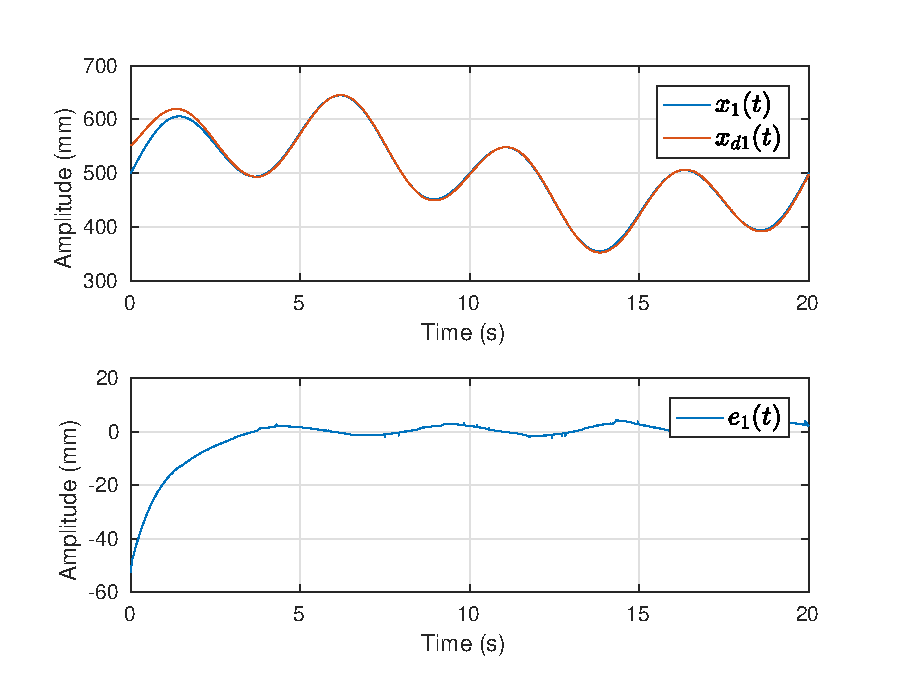
\includegraphics[width=\linewidth]{./img/trk1/x1.eps}
  \caption{$x_1$, $x_{d1}$ e $e_1$}
  \label{fig:sub1}
\end{subfigure}%
\begin{subfigure}{.5\textwidth}
  \centering
  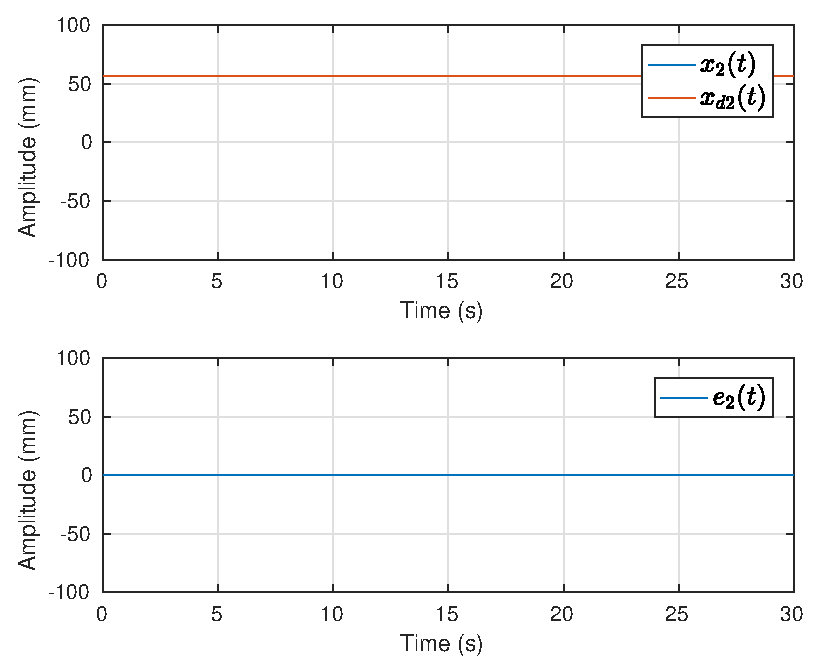
\includegraphics[width=\linewidth]{./img/trk1/x2.eps}
  \caption{$x_2$, $x_{d2}$ e $e_2$}
  \label{fig:sub2}
\end{subfigure}
\begin{subfigure}{.5\textwidth}
  \centering
  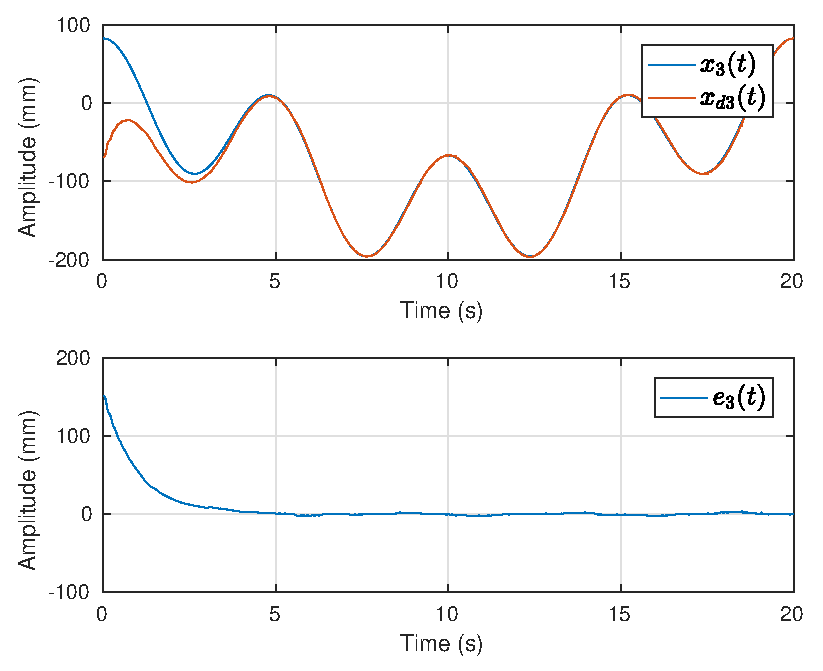
\includegraphics[width=\linewidth]{./img/trk1/x3.eps}
  \caption{$x_3$, $x_{d3}$ e $e_3$}
  \label{fig:sub1}
\end{subfigure}%
\begin{subfigure}{.5\textwidth}
  \centering
  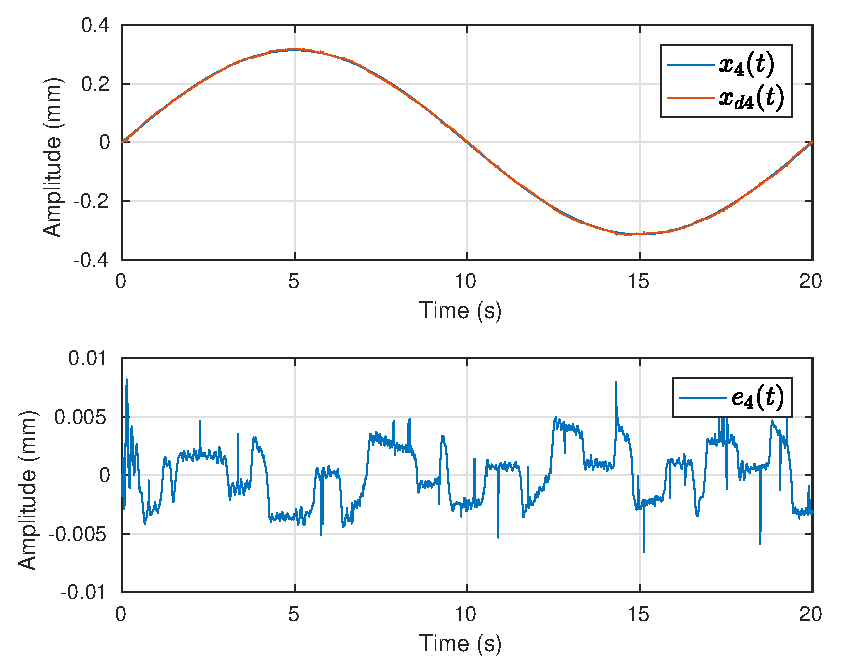
\includegraphics[width=\linewidth]{./img/trk1/x4.eps}
  \caption{$x_4$, $x_{d4}$ e $e_4$}
  \label{fig:sub2}
\end{subfigure}
\caption{A figure with two subfigures}
\label{fig:test}
\end{figure}


  \chapter{Conclusões e Trabalhos Futuros}

\section{Conclusões}

Neste projeto de graduação foi apresentada a modelagem cinemática, estratégias de controle baseadas na abordagem de controle cinemático, assim como a implementação de um software para controle de sistemas robóticos, utilizando como estudo de caso o manipulador TETIS, do sistema DORIS. 

A modelagem cinemática consiste em representar o manipulador como uma cadeia cinemática de corpos rígidos, de modo a obter relações geométricas que governam o sistema. A cinemática direta do manipulador TETIS foi obtida através da convenção Denavit–Hartenberg. Diferenciando as equações resultantes com respeito as variáveis das juntas foi possível obter a cinemática diferencial, relacionando a velocidade no espaço operacional com as variáveis de juntas, na forma do Jacobiano analítico. Em simulação os resultados se mostraram compatíveis com o esperado. 

A abordagem de controle cinemático assume que é possível considerar um sistema cinemático como entrada do sistema, tipicamente um valor de velocidade. Isso é possível quando existe uma malha de controle de baixo nível, que idealmente é capaz de impor uma velocidade especificada de referência. Esse é o caso do TETIS, que utiliza atuadores \textit{FHA Mini Servo} com drivers EPOS2 70/10, com uma malha de baixo nível de velocidade. Assim, utilizou-se como modelo simplificado do robô um integrador, supondo que os servos são capazes de reproduzir comandos de velocidade de forma razoavelmente precisa. No caso da junta 2, essa reprodução não é tão precisa devido necessidade de maior torque, por estar no início da cadeia.

O rastreamento de trajetória com controle proporcional com \textit{feedforward} apresentou erro em regime permanente pelos seguintes fatores: (i) ciclo de controle máximo que o computador embarcado suporta é de $10ms$; (ii) Junta 2 não é capaz de reproduzir com tanta precisão comandos de velocidade, por estar mais sujeita à força gravitacional; (iii) Ciclo de controle está sujeito a atrasos devido a interrupções do sistema operacional. 

Os componentes de software para controle, interação e configuração de parâmetros foram desenvolvidos e integrados ao RobotGUI, que já era utilizado para controle dos demais sistemas do robô. A interface gráfica permite a visualização de dados de forma gráfica \textit{online} dos sinais, assim como a reconfiguração de parâmetros no computador embarcado com aquelas desejadas. A adição de novas funcionalidades e modos de controle é imediata, devido a arquitetura modular e ao paradigma orientado a objetos. O ROS segue os princípios de um microkernel, onde as funcionalidades são implementadas separadamente em módulos bem definidos que se comunicam, em contraste com um "monolito" que realiza todas as funções. Isso permite que nós possam ser substituidos ou modificados sem influenciar outros, desde que sigam o mesmo protocolo (tópicos/serviços). Por exemplo, caso seja de interesse substituir o módulo de visão computacional basta publicar/subscrever aos mesmos tópicos.

A implementação de software para controle com computação em tempo real é custosa em tempo de implementação e pouco expansível, necessitando tratar de algoritmos de \textit{scheduling} e latência de entrada/saída \citep{nilsson1998real}. A abordagem utilizada neste trabalho permite uma implementação mais desacoplada e menos interdependente. No entanto, existem algumas desvantagens do uso do ROS para um software completamente desacoplado. Existem \textit{overheads} de comunicação entre \textit{ROS Nodes}, que pode se tornar crítico no caso de separar o nó de controle do nó de atuação, conforme mostrado no apêndice \ref{chap:delay}. Essa separação introduziria atrasos significativos, tornando-se evidente para o caso em que o objetivo de controle é rastrear uma trajetória que é função do tempo. Em casos como nó de visão computacional que realiza o processamento de imagem a separação é inevitável e não representa um problema. Conclui-se ser mais apropriado juntar os nós de atuação e controle, o que melhorou significativamente o erro de rastreamento. %, já que o tempo de processamento já é 

Com o uso do Julia Language foi possível alterar em tempo de execução a trajetória a ser rastreada escrevendo as equações em uma janela na interface, com uma sintaxe simples. O \textit{script} é compilado \textit{just-in-time} e pode ser executado sem perda de performance.
%Com base nos resultados obtidos:
%Quando se necessita de ROS nem sempre é uma solução adequada,

\section{Trabalhos futuros}
\begin{itemize}
\item Modelo dinâmico do manipulador TETIS.

\item Utilizar ambos os sensores da cãmera estereoscópica Minoru de modo a melhorar a estimação da posição e orientação de um alvo, assim como ampliar o campo de visão.

\item Extender o uso do Julia Language, de modo a tornar o controle ainda mais dinâmico. Atualmente é utilizado somente na definição de uma trajetória a ser rastreada, no entanto é possível implementar algoritmos de controle inteiramente no Julia, o que permitiria ajustes e experimentos em tempo de execução.

\item Estudar implementações para sistemas de controle em tempo real e como tratar atrasos de entrada/saída.
\item Integrar o \textit{Sensable Phantom Omni}, um dispositivo háptico, em modo Master/Slave.
\end{itemize}

%A cinemática direta expressa a posição e orientação do efetuador final em função das variáveis de junta, enquanto que a cinemática diferencial fornece a relação entre a velocidade das juntas e a velocidade do efetuador final.

  
  \backmatter
  \bibliographystyle{coppe-unsrt}
  \bibliography{thesis}

  \appendix
  %\chapter{Algumas Demonstra{\c c}\~oes}
%\chapter{Estimação da posição e orientação}
\chapter{Estimação da \textit{pose} em tempo real} 
 
\section{ViSP - Visual Servoing Platform}

Para a implementação do modo de controle por Servo Visão, foi utilizada a biblioteca ViSP. A ViSP contém um módulo de visão computacional que permite computar a \textit{pose} de um objeto a ser reconhecido por meio de um padrão pre-determindado. São utilizados algoritmos robustos e fornecidos mecanismos para calibração da câmera. Esse módulo é um envoltório para a biblioteca OpenCV com algoritmos focados em aplicações de robótica.

\begin{itemize}
\item Linear Lagrange approach (test is done to switch between planar and non planar algorithm)
\item Linear Dementhon approach (test is done to switch between planar and non planar algorithm)
\item Lowe aproach based on a Levenberg Marquartd non linear minimization scheme that needs an initialization from Lagrange or Dementhon aproach
\item  Non linear Lowe aproach initialized by Lagrange approach
\end{itemize}

\section{OpenCV}

\end{document}